\documentclass[12pt,a4paper]{article}

\usepackage[a4paper,margin=1in]{geometry}
\usepackage{graphicx}
\usepackage{booktabs}
\usepackage{amsmath,amssymb}
\usepackage{float}
\usepackage{hyperref}
\usepackage{xcolor}
\usepackage{listings}
\usepackage{enumitem}
\usepackage{fancyhdr}
\usepackage{longtable}

\hypersetup{colorlinks=true,linkcolor=blue,urlcolor=blue}

\pagestyle{fancy}
\fancyhf{}
\lhead{ICS1512}
\rhead{Machine Learning Algorithms Laboratory}
\cfoot{\thepage}

\lstset{
language=Python,
basicstyle=\ttfamily\small,
numbers=left,
frame=single,
breaklines=true,
showstringspaces=false
}

\begin{document}

\begin{tabular}{|p{4cm}|p{11cm}|}
\hline
Experiment No. & 1 \\ \hline
Experiment Title & Working with Python packages -- NumPy, SciPy, Scikit-Learn,
Matplotlib\footnotemark\\ \hline
Student Name & Simiyon Vinscent Samuel L \\ \hline
Register Number & 3122247001062 \\ \hline
Faculty & Dr. Poreddy Ajay Kumar Reddy \\ \hline
Submission Date & August 2, 2026 \\ \hline
\end{tabular}
\footnotetext{\textbf{GitHub Repository: }\url{https://github.com/blackscythe123/Machine-Learning-course}}

\section{Objective}
To explore the core functions of NumPy, Pandas, SciPy, Scikit-learn and Matplotlib, and
to survey five reference datasets in order to identify the type of machine learning task
(supervised/unsupervised, classification/regression), a suitable feature-selection
technique, and a suitable algorithm for each.

\section{Problem Statement}
This experiment has two parts. Part A explores the core functions of five Python
data-science libraries (NumPy, Pandas, SciPy, Scikit-learn, Matplotlib) that the rest of
this laboratory course builds on. Part B surveys five reference datasets (Iris, Loan
Amount Prediction, Pima Indians Diabetes, Spambase, and the \texttt{digits}
handwritten-character dataset) to identify, for each, the appropriate machine learning
task type (supervised/unsupervised, classification/regression), a suitable
feature-selection technique, and a suitable algorithm family. Unlike Experiments 2--4, no
single model is trained or tuned here; the goal is a working familiarity with the
tooling and a taxonomy of techniques that motivates the modelling choices made in the
later experiments.

\section{Dataset Description}
\begin{longtable}{|p{4cm}|p{2.2cm}|p{2.8cm}|p{6cm}|}
\hline
\textbf{Dataset} & \textbf{Samples} & \textbf{Features} & \textbf{Classes / Target} \\ \hline
Iris & 150 & 4 numeric & 3 classes (species) \\ \hline
Loan Amount Prediction & 614 applications (149 missing values across all columns) & 5
numeric + 5 categorical & Continuous target (\texttt{LoanAmount}) \\ \hline
Pima Indians Diabetes & 768 & 8 numeric & 2 classes (500 negative / 268 positive) \\ \hline
Spambase & 4601 emails & 57 numeric, 0 missing & 2 classes (spam / ham) \\ \hline
\texttt{digits} (MNIST stand-in) & 1797 & 64 (8$\times$8 pixel intensities) & 10 classes
(digits 0--9) \\ \hline
\end{longtable}

\section{Exploratory Data Analysis}

\subsection*{Iris Dataset}
\begin{figure}[H]
\centering
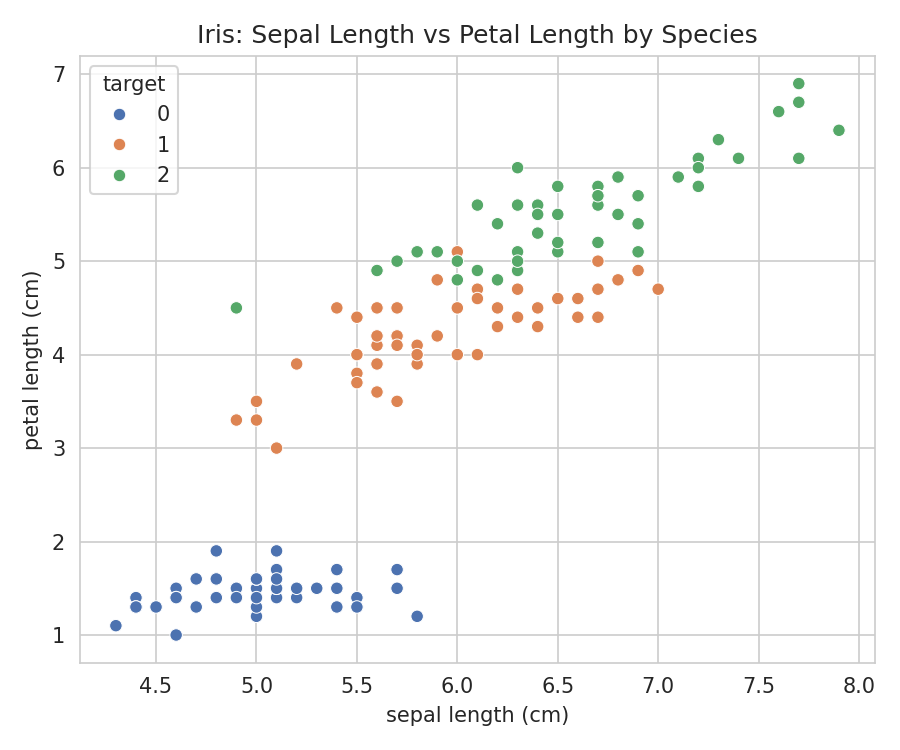
\includegraphics[width=0.55\linewidth]{figures/01_iris_scatter.png}
\caption{Iris: sepal length vs.\ petal length, coloured by species (150 samples, 4
features, 3 classes).}
\end{figure}
\textbf{Inference:} \textit{Setosa} is linearly separable from the other two species on
this feature pair alone; \textit{versicolor} and \textit{virginica} overlap slightly,
which is why simple linear classifiers already achieve high accuracy on Iris but a
non-linear boundary helps at the versicolor/virginica margin.

\subsection*{Loan Amount Prediction}
\begin{figure}[H]
\centering
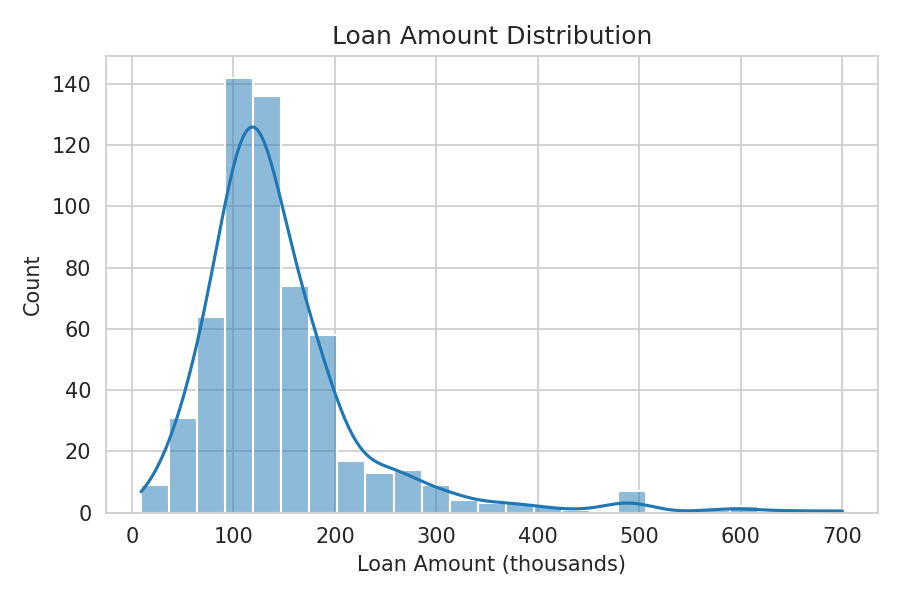
\includegraphics[width=0.55\linewidth]{figures/02_loan_hist.png}
\caption{Distribution of \texttt{LoanAmount} (614 applications, 149 missing values
across all columns).}
\end{figure}
\textbf{Inference:} The right-skewed target and the mix of 5 numeric + 5 categorical
features (with real missing values) make this a regression task requiring both
imputation and categorical encoding, which is exactly the pipeline built in Experiment 3.

\subsection*{Predicting Diabetes}
\begin{figure}[H]
\centering
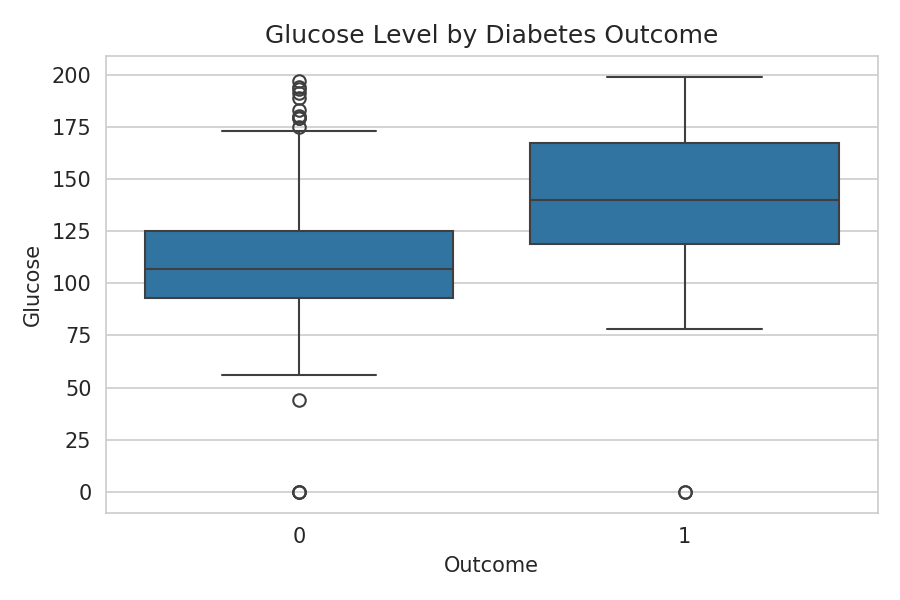
\includegraphics[width=0.55\linewidth]{figures/03_diabetes_box.png}
\caption{Glucose level by diabetes outcome (Pima Indians Diabetes dataset, 768 samples,
class balance 500 negative / 268 positive).}
\end{figure}
\textbf{Inference:} Glucose level shows a clear separation between the two outcome
classes (higher median and higher spread for the diabetic group), making it, along with
BMI and Age, one of the strongest univariate predictors identified by the ANOVA F-test.

\subsection*{Classification of Email Spam}
\begin{figure}[H]
\centering
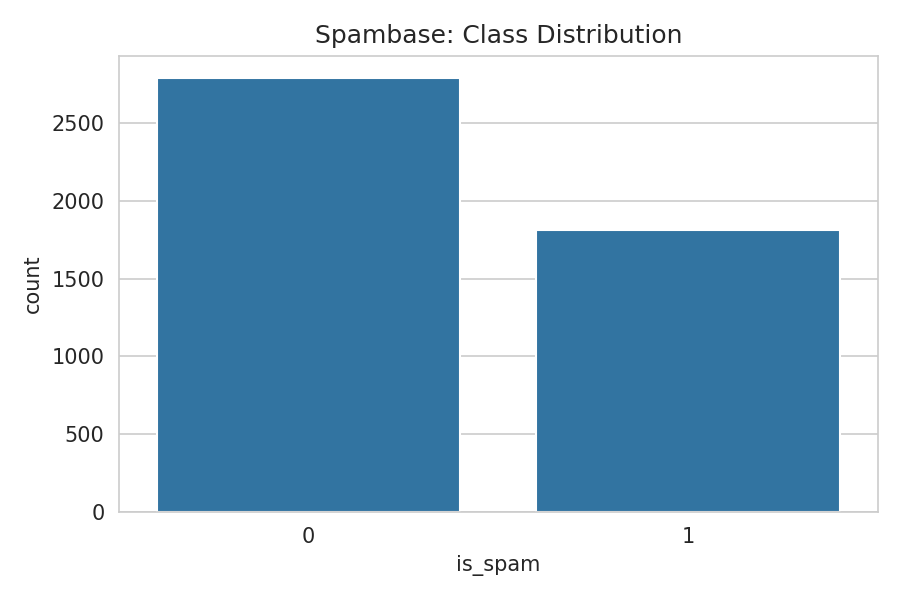
\includegraphics[width=0.5\linewidth]{figures/04_spam_countplot.png}
\caption{Spambase class distribution (4601 emails, 57 numeric features, 0 missing
values).}
\end{figure}
\textbf{Inference:} This is a moderately imbalanced binary classification task on
purely numeric, non-negative frequency features (the same dataset used and analyzed in
depth in Experiments 2 and 4).

\subsection*{Handwritten Character Recognition / MNIST}
\begin{figure}[H]
\centering
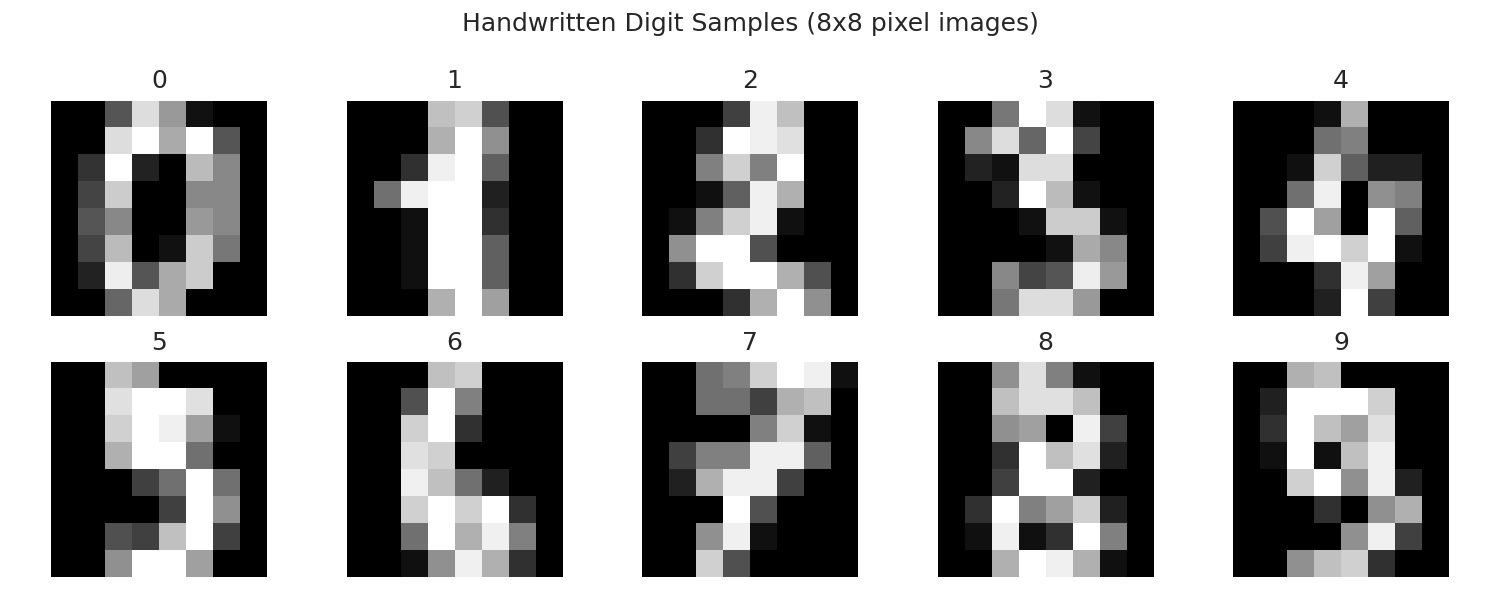
\includegraphics[width=0.75\linewidth]{figures/05_digits_samples.png}
\caption{Sample handwritten digit images (8$\times$8 pixel \texttt{digits} dataset, 1797
samples, 10 classes, used here as a lightweight, fully offline stand-in for the larger
28$\times$28 MNIST benchmark, since both pose the identical multi-class image
classification task).}
\end{figure}
\textbf{Inference:} Each image is a 64-dimensional pixel-intensity vector; the high
dimensionality relative to sample count is the classic motivation for PCA-based
dimensionality reduction before applying distance-based classifiers such as k-NN or SVM.

\section{Data Preprocessing}
Preprocessing needs identified per dataset (implemented in full in the experiments that
model them):
\begin{itemize}
\item \textbf{Missing-value handling} -- required for Loan Amount Prediction (149 missing
values across columns); Iris, Spambase and \texttt{digits} are clean (imputation-free) by
construction, and Diabetes is used here in its raw form.
\item \textbf{Categorical encoding} -- required for Loan Amount Prediction (5 categorical
features); the other four datasets are purely numeric.
\item \textbf{Feature standardization} -- appropriate for all numeric-feature datasets
before applying scale-sensitive algorithms such as KNN, SVM or PCA.
\end{itemize}
No single preprocessing pipeline is executed in this experiment; each dataset's specific
preprocessing is implemented and evaluated in the experiment where it is modelled (Loan
$\to$ Experiment 3; Spambase $\to$ Experiments 2 and 4).

\section{Machine Learning Algorithm}

\subsection*{NumPy}
Explored array creation, reshaping, and vectorized operations:
\begin{lstlisting}
a = np.arange(12).reshape(3, 4)
a.sum(), a.mean(), a.std()   # 66, 5.5, 3.452
a.T                          # transpose
a @ a.T                      # matrix product
\end{lstlisting}
\textbf{Inference:} NumPy's vectorized operations (\texttt{sum}, \texttt{mean},
\texttt{@} for matrix multiplication) avoid explicit Python loops and are the
computational backbone that Pandas and Scikit-learn are built on.

\subsection*{Pandas}
Explored \texttt{DataFrame} construction, \texttt{groupby}, and \texttt{describe}:
\begin{lstlisting}
df.groupby("category").mean(numeric_only=True)
df.describe()
\end{lstlisting}
\textbf{Inference:} \texttt{groupby} is the primary tool for computing per-category
statistics, and \texttt{describe()} gives a fast statistical summary (count, mean, std,
quartiles) that is normally the first step of any EDA.

\subsection*{SciPy}
Explored hypothesis testing (\texttt{scipy.stats}) and linear algebra
(\texttt{scipy.linalg}):
\begin{lstlisting}
t_stat, p_val = stats.ttest_ind(group_A, group_B)   # t=-0.094, p=0.928
eigvals, eigvecs = linalg.eig(matrix)                # [5.0, 2.0]
\end{lstlisting}
\textbf{Inference:} An independent two-sample $t$-test on the synthetic demo groups gave
$p=0.928$, correctly indicating no significant difference (the two groups were drawn
from the same distribution by construction). \texttt{scipy.linalg.eig} confirmed the
eigenvalues of a simple $2\times2$ matrix, illustrating SciPy's role as the numerical
layer beneath many ML algorithms (e.g.\ PCA relies on eigendecomposition).

\subsection*{Scikit-learn}
Explored \texttt{SelectKBest} for univariate feature selection:
\begin{lstlisting}
SelectKBest(score_func=f_classif, k=2).fit(iris.data, iris.target).scores_
# [119.26, 49.16, 1180.16, 960.01]
\end{lstlisting}
\textbf{Inference:} On the Iris dataset, petal length and petal width (F-scores 1180.16
and 960.01) are far more discriminative between species than sepal length and width
(119.26 and 49.16), matching the well-known fact that petal measurements separate Iris
species much more cleanly than sepal measurements.

\subsection*{Matplotlib}
\begin{figure}[H]
\centering
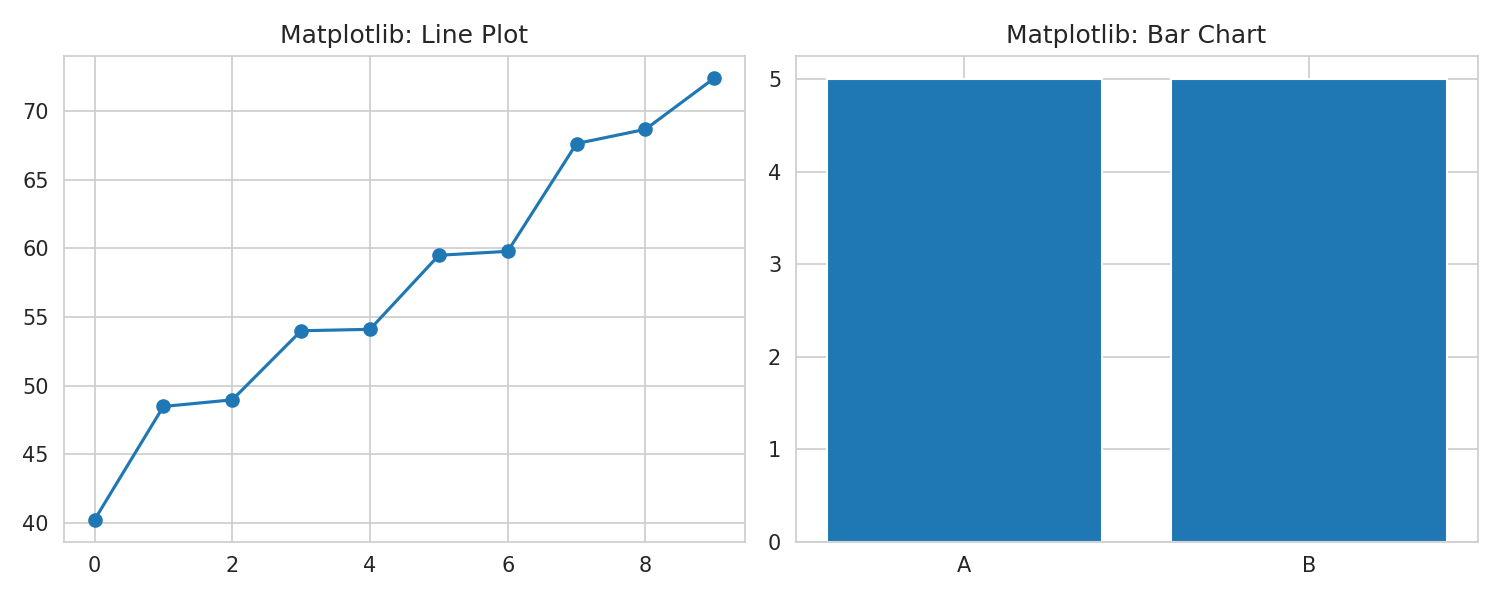
\includegraphics[width=0.85\linewidth]{figures/00_library_demo.png}
\caption{Matplotlib line plot and bar chart generated from the demonstration DataFrame.}
\end{figure}
\textbf{Inference:} \texttt{plt.subplots} is the standard way to lay out multiple axes in
one figure, used throughout Experiments 2--4 for combining several related plots into a
single saved image.

\subsection*{Summary: Dataset $\rightarrow$ ML Task $\rightarrow$ Feature Selection $\rightarrow$ Algorithm}
\begin{longtable}{|p{3.2cm}|p{3.6cm}|p{3.6cm}|p{3.6cm}|}
\hline
\textbf{Dataset} & \textbf{Type of ML Task} & \textbf{Feature Selection Technique} &
\textbf{Suitable ML Algorithm} \\ \hline
Iris Dataset & Supervised -- Multi-class Classification & ANOVA F-test / SelectKBest
(all 4 features informative; petal features dominate) & Logistic Regression / KNN / SVM
\\ \hline
Loan Amount Prediction & Supervised -- Regression (continuous target) & Correlation
analysis + domain-driven selection (income, credit history) & Linear / Ridge / Lasso /
Elastic Net Regression \\ \hline
Predicting Diabetes & Supervised -- Binary Classification & ANOVA F-test (top: Glucose,
BMI, Age, Pregnancies) & Logistic Regression / Random Forest / SVM \\ \hline
Classification of Email Spam & Supervised -- Binary Classification & Correlation with
label + variance threshold (57 numeric features) & Naive Bayes / KNN / Logistic
Regression / SVM \\ \hline
Handwritten Character Recognition / MNIST & Supervised -- Multi-class Classification
(10 classes) & PCA (dimensionality reduction on pixel features) & CNN / SVM (RBF
kernel) / Random Forest / k-NN \\ \hline
\end{longtable}

\section{Experimental Setup}
\begin{tabular}{ll}
\toprule
Python Version & 3.12.3 \\
Scikit-Learn Version & 1.8.0 \\
IDE & Jupyter Notebook \\
Operating System & Windows 11 \\
Hardware & Intel Core Ultra 9, NVIDIA RTX 5060 \\
\bottomrule
\end{tabular}

\section{Hyperparameter Selection}
\textit{Not applicable.} This experiment surveys library functions and five reference
datasets to identify appropriate tasks, feature-selection techniques and algorithms; it
does not train or tune a single model, so no hyperparameter search was performed.
Hyperparameter tuning for these same datasets and algorithm families is carried out in
Experiments 2--4.

\section{Results}
\textit{Not applicable.} No model is trained or evaluated in this experiment, so there
are no accuracy/precision/recall-style results to report. The closest analogue is the
dataset $\to$ task $\to$ technique $\to$ algorithm summary table in Section 6 (Machine
Learning Algorithm).

\section{Result Visualization}
\textit{Not applicable in the usual sense}, since there is no trained model to visualize
results for. This experiment's visualizations are exploratory rather than post-model, and
are presented in Section 4 (Exploratory Data Analysis) instead.

\section{Discussion}
Across all five datasets, the same general machine learning workflow recurs:
\begin{enumerate}[nosep]
\item \textbf{Loading the dataset} -- from CSV / library loaders (\texttt{sklearn.datasets}).
\item \textbf{EDA and visualization} -- histograms, scatter plots, boxplots, count
plots, as shown in Section 4 for each dataset.
\item \textbf{Data preprocessing} -- missing value handling (Loan, Diabetes), encoding
categorical variables (Loan), and standardization (all numeric-feature datasets).
\item \textbf{Feature selection} -- \texttt{SelectKBest}/ANOVA F-test for the
classification datasets, correlation analysis for the regression dataset, and PCA for
the high-dimensional image dataset.
\item \textbf{Data splitting} -- stratified train/test (and cross-validation) splits, as
applied throughout Experiments 2--4.
\item \textbf{Performance evaluation} -- accuracy/precision/recall/F1/ROC-AUC for
classification tasks; MAE/MSE/RMSE/$R^2$ for the regression task.
\end{enumerate}
Every later experiment in this course follows these same six steps, differing only in
which preprocessing, feature-selection and algorithm choices apply to its specific
dataset.

\section{Conclusion}
This experiment built working familiarity with the core Python data-science stack
(NumPy, Pandas, SciPy, Scikit-learn, Matplotlib) and produced a task/technique/algorithm
taxonomy for five reference datasets spanning multi-class classification, regression,
binary classification and high-dimensional image classification. No single model was
trained here; instead, the experiment built the library familiarity, task-identification
skills, and reusable six-step workflow that Experiments 2--4 use directly.

This experiment also reinforced the following learning outcomes:
\begin{itemize}[nosep]
\item Gained hands-on familiarity with NumPy, Pandas, SciPy, Scikit-learn and Matplotlib
as the core Python data-science stack.
\item Learned to distinguish supervised classification, supervised regression and
image-based classification tasks from a dataset's feature types and target variable.
\item Understood how feature-selection technique choice depends on data type (ANOVA
F-test for continuous features vs.\ a classification target; PCA for high-dimensional
pixel data).
\item Recognized the machine learning workflow (load $\to$ EDA $\to$ preprocess $\to$
select features $\to$ split $\to$ evaluate) as a common pattern reused across all
subsequent experiments in this laboratory course.
\end{itemize}

\section{References}
\begin{enumerate}
\item NumPy Developers, \url{https://numpy.org/doc/}
\item Pandas Developers, \url{https://pandas.pydata.org/docs/}
\item SciPy Developers, \url{https://docs.scipy.org/doc/scipy/}
\item Scikit-learn Developers, \url{https://scikit-learn.org/stable/}
\item Matplotlib Developers, \url{https://matplotlib.org/stable/}
\item UCI Machine Learning Repository, \url{https://archive.ics.uci.edu/}
\item Kaggle Datasets, \url{https://www.kaggle.com/datasets}
\end{enumerate}

\end{document}
